% Chapter 3: The Second Fundamental Form and the Geometry of Surfaces
\chapter{The Second Fundamental Form and Local Surface Theory}\label{chap:ch3}

% ==================== Section 3-1: The Second Fundamental Form ====================
\section{The Second Fundamental Form}\label{sec:second-fundamental-form}

\textbf{From the first to the second fundamental form.} 在第二章中，我们研究了曲面的第一基本形式 $I = Edu^2 + 2Fdudv + Gdv^2$，它源自曲面的切平面结构——切向量之间的内积。第一基本形式完全决定了曲面上的度量性质：弧长、面积、角度。

但这只是故事的一半。曲面的"弯曲"程度——即它如何偏离切平面——需要另一个量来描述，这就是\textbf{第二基本形式}（second fundamental form）。

\textbf{Why do we need a second form?} 考虑一个具体的问题：给定曲面 $S$ 上一点 $p$ 和一个切方向 $v$，曲面在 $p$ 点沿方向 $v$ 是向上弯还是向下弯？第一基本形式只告诉我们方向和长度，无法回答这个问题。

要测量"偏离切平面"的程度，我们需要考虑二阶信息。直观上，第二基本形式衡量的是曲面在法向上的二阶变化。

\begin{Definition}[第二基本形式]\label{def:second-fundamental-form}
设 $S \subset \mathbb{R}^3$ 是正则曲面，$N$ 是单位法向量场。曲面在点 $p$ 处的\textbf{\underline{第二基本形式}}（second fundamental form）是切空间上的二次型
\[
\II_p(v, w) = \langle S_p(v), w \rangle = \langle dN_p(v), w \rangle,
\]
其中 $S_p: T_pS \to T_pS$ 是 Weingarten 映射（见 \cref{sec:weingarten-map}）。
\end{Definition}

\textbf{Coefficients.} 在参数化 $\mathbf{x}(u,v)$ 下，第二基本形式可以写成
\[
\II = L\,du^2 + 2M\,dudv + N\,dv^2,
\]
其中
\[
L = \langle \mathbf{x}_{uu}, N \rangle,\quad M = \langle \mathbf{x}_{uv}, N \rangle,\quad N = \langle \mathbf{x}_{vv}, N \rangle.
\tag{3-1}
\]

这里 $\mathbf{x}_{uu} = \partial^2\mathbf{x}/\partial u^2$ 等是参数化的二阶偏导数，$N$ 是单位法向量
\[
N = \frac{\mathbf{x}_u \times \mathbf{x}_v}{\|\mathbf{x}_u \times \mathbf{x}_v\|}.
\tag{3-2}
\]

\begin{Remark}[几何意义]
第一基本形式 $I$ 衡量切平面上的内积——它测量曲面作为度量空间的结构。
第二基本形式 $\II$ 衡量曲面如何"离开"切平面——它测量曲面作为嵌入 $\mathbb{R}^3$ 的子流形的弯曲程度。

这两个基本形式共同决定了曲面的全部局部几何。
\end{Remark}

\begin{Example}[平面的第二基本形式]\label{ex:plane-second-form}
设 $S$ 是 $xy$ 平面，参数化为 $\mathbf{x}(u,v) = (u,v,0)$。则
\[
\mathbf{x}_u = (1,0,0),\quad \mathbf{x}_v = (0,1,0),\quad N = (0,0,1).
\]
由于所有二阶导数为零，$L = M = N = 0$。平面的第二基本形式恒为零——平面完全不弯曲。
\end{Example}

\begin{Example}[球面的第二基本形式]\label{ex:sphere-second-form}
单位球面 $S^2$ 在地理坐标下的参数化为
\[
\mathbf{x}(\theta,\varphi) = (\sin\theta\cos\varphi,\; \sin\theta\sin\varphi,\; \cos\theta).
\]
直接计算（见 \cref{sec:ch3-derivations}）可得
\[
L = -1,\quad M = 0,\quad N = -\sin^2\theta.
\tag{3-3}
\]
球面上 $S_p = -I$（Weingarten 映射是恒等变换的负值），故 $\kappa_1 = \kappa_2 = -1$，这与 $L, M, N$ 的值一致——球面是全脐点（totally umbilic）曲面。
\end{Example}

\begin{Example}[旋转抛物面的第二基本形式]\label{ex:paraboloid-second-form}
考虑旋转抛物面 $z = x^2 + y^2$，参数化为 $\mathbf{x}(u,v) = (u, v, u^2+v^2)$。计算得
\[
L = \frac{2}{\sqrt{1+4(u^2+v^2)}},\quad M = 0,\quad N = \frac{2}{\sqrt{1+4(u^2+v^2)}}.
\tag{3-4}
\]
在原点处，$L=N=2$，$M=0$。
\end{Example}

\textbf{An important observation.} 第二基本形式的系数依赖于法向量的选择。如果选择相反的法向量方向 $-N$，则 $L, M, N$ 全部变号。因此，第二基本形式的符号在定向改变时会反转——但其零迹（zero set）和特征值（主曲率）不受影响。

\begin{figure}[H]
\centering
\subfloat[Figure 3-1. The Möbius strip — 不可定向曲面的经典例子]{\label{fig:fig3-1}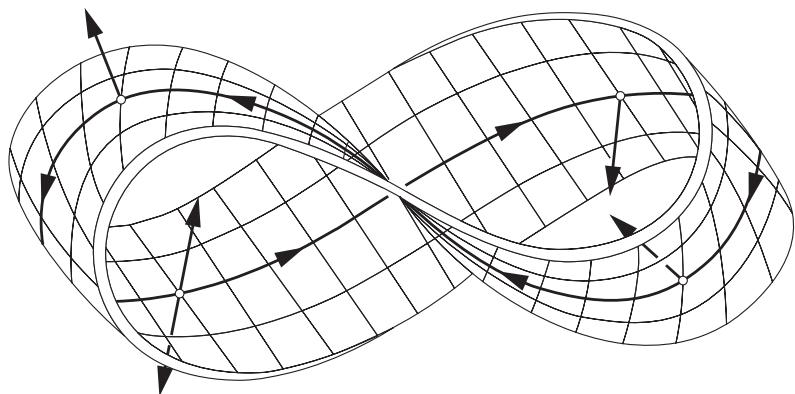
\includegraphics[width=0.6\textwidth]{../../../PDFs/differential-geometry/transcript/Do Carmo - Differential Geometry of Curves and Surfaces/hybrid_ocr/images/53c3f147d73fbbaff460736e7109c90902470b480130ac9116222c530a8f7b29.jpg}}
\end{figure}

% ==================== Section 3-2: The Weingarten Map ====================
\section{The Weingarten Map (Shape Operator)}\label{sec:weingarten-map}

\textbf{From Gauss map to shape operator.} 在第二章中，我们引入了 Gauss 映射 $N: S \to S^2$，它将曲面上每一点映射到单位球面上对应的法向量。Gauss 映射的微分 $dN_p: T_pS \to T_{N(p)}S^2$ 将切向量映射到球面上的切向量。

但 $T_{N(p)}S^2$ 与 $T_pS$ 是同一个平面（两者都垂直于 $N(p)$）！因此，我们可以将 $dN_p$ 视为 $T_pS$ 上的线性变换。

\begin{Definition}[Weingarten 映射]\label{def:weingarten-map}
设 $S \subset \mathbb{R}^3$ 是可定向的正则曲面，$N: S \to S^2$ 是单位法向量场。点 $p$ 处的\textbf{\underline{Weingarten 映射}}（Weingarten map）或\textbf{\underline{形状算子}}（shape operator）为
\[
S_p = -dN_p: T_pS \to T_pS.
\tag{3-5}
\]
负号是历史惯例，使得 $S_p$ 在法曲率计算中有一个自然的解释。
\end{Definition}

Weingarten 映射是曲面论的核心工具。它建立了两个基本形式之间的联系：

\begin{Proposition}[两个基本形式的关系]\label{prop:second-form-weingarten}
对任意 $v, w \in T_pS$，有
\[
\II_p(v, w) = \langle S_p(v), w \rangle = I_p(S_p(v), w).
\tag{3-6}
\]
\end{Proposition}

这个命题表明：给定第一基本形式的系数 $E, F, G$ 和 Weingarten 映射在基底下的矩阵，我们可以计算第二基本形式。反过来，给定两个基本形式的系数，我们可以确定 $S_p$。

在参数化基底下，$S_p$ 的矩阵为
\[
S_p = \begin{pmatrix} E & F \\ F & G \end{pmatrix}^{-1} \begin{pmatrix} L & M \\ M & N \end{pmatrix}.
\tag{3-7}\label{eq:matrix-representation}
\]

\textbf{Key property.} Weingarten 映射是自共轭的（self-adjoint）——这意味着它关于第一基本形式的内积是对称的：
\[
\langle S_p(v), w \rangle = \langle v, S_p(w) \rangle.
\tag{3-8}
\]
这一性质确保了 $S_p$ 有实特征值和两两正交的特征方向。

\begin{figure}[H]
\centering
\begin{minipage}{0.48\textwidth}
\centering
\subfloat[Figure 3-2. The Gauss map $N: S \to S^2$]{\label{fig:fig3-2}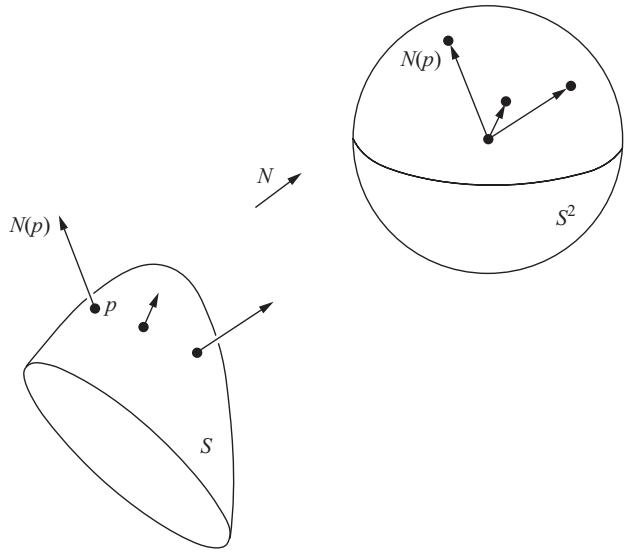
\includegraphics[width=\textwidth]{../../../PDFs/differential-geometry/transcript/Do Carmo - Differential Geometry of Curves and Surfaces/hybrid_ocr/images/216853bb9c9d2a1d4811f2cd06eea0b1ea035c4b263de20ca9c903b47accf589.jpg}}
\end{minipage}
\hfill
\begin{minipage}{0.48\textwidth}
\centering
\subfloat[Figure 3-3. $dN_p$ 的几何意义]{\label{fig:fig3-3}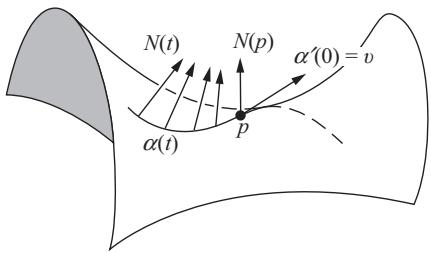
\includegraphics[width=\textwidth]{../../../PDFs/differential-geometry/transcript/Do Carmo - Differential Geometry of Curves and Surfaces/hybrid_ocr/images/fa20784ffa0cf87b26556fefc3048146f0287308bc09e31a93cf962aa4714cf4.jpg}}
\end{minipage}
\end{figure}

\begin{figure}[H]
\centering
\begin{minipage}{0.48\textwidth}
\centering
\subfloat[Figure 3-4. Plane: $dN_p = 0$]{\label{fig:fig3-4}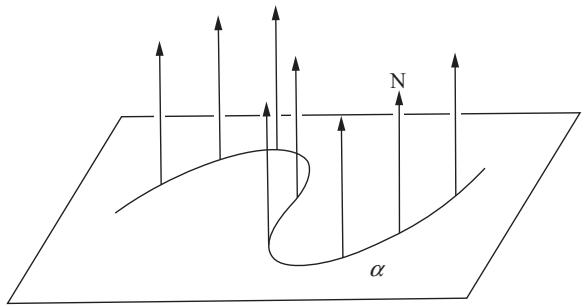
\includegraphics[width=\textwidth]{../../../PDFs/differential-geometry/transcript/Do Carmo - Differential Geometry of Curves and Surfaces/hybrid_ocr/images/f6b49975c2896eba1d8c302e6ea2aacff718212b7aa3cc41b9d9a8de01a2b3bc.jpg}}
\end{minipage}
\hfill
\begin{minipage}{0.48\textwidth}
\centering
\subfloat[Figure 3-5. Unit sphere: $d\bar{N}_p(v) = v$]{\label{fig:fig3-5}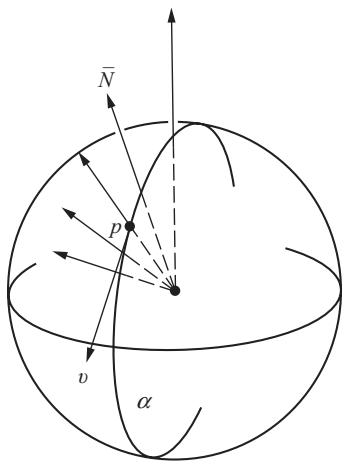
\includegraphics[width=\textwidth]{../../../PDFs/differential-geometry/transcript/Do Carmo - Differential Geometry of Curves and Surfaces/hybrid_ocr/images/c0ffa599c2b6e7a0e2c8b098970dfcc6ec6474b8b6c2b0a1a998e43e4a126acf.jpg}}
\end{minipage}
\end{figure}

\begin{figure}[H]
\centering
\subfloat[Figure 3-6. 圆柱面的 $dN$]{\label{fig:fig3-6}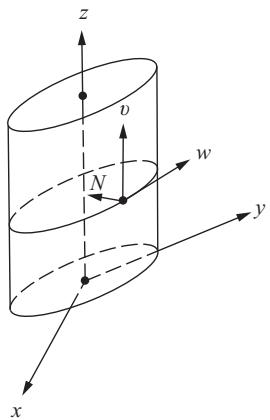
\includegraphics[width=0.6\textwidth]{../../../PDFs/differential-geometry/transcript/Do Carmo - Differential Geometry of Curves and Surfaces/hybrid_ocr/images/7e110dac56ae33192bfe686568e285d52b2bcf6e289089bc6e98471f331ffa9e.jpg}}
\end{figure}

% ==================== Section 3-3: Normal Curvature ====================
\section{Normal Curvature}\label{sec:normal-curvature}

\textbf{Why normal curvature?} 给定曲面上一点 $p$ 和一个切方向 $v$，我们想知道曲面在该方向上的"弯曲程度"。法曲率 $\kappa_n$ 正是这个问题的答案——它描述了曲面在给定方向上如何偏离切平面。

\begin{Definition}[法曲率]\label{def:normal-curvature}
设 $p \in S$，$v \in T_pS$ 是单位切向量。沿方向 $v$ 的\textbf{\underline{法曲率}}（normal curvature）为
\[
\kappa_n(p, v) = \II_p(v, v) = \langle S_p(v), v \rangle.
\tag{3-9}
\]
\end{Definition}

法曲率的几何意义可以通过以下方式理解：取经过 $p$ 点、方向为 $v$ 的测地线 $\gamma$，将 $\gamma$ 投影到法平面（由 $v$ 和 $N$ 张成）中，得到一条平面曲线 $\tilde{\gamma}$。则 $\kappa_n = \kappa_{\tilde{\gamma}}$，即 $\tilde{\gamma}$ 的曲率。

\begin{Proposition}[Meusnier 定理]\label{prop:meusnier}
所有经过 $p$ 点、方向为 $v$ 的曲线在 $p$ 点有相同的法曲率 $\kappa_n(p, v)$。
\end{Proposition}

Meusnier 定理告诉我们：法曲率只依赖于方向 $v$，而不依赖于具体曲线的选择。这是曲面内蕴几何的一个体现。

\begin{Example}[平面的法曲率]\label{ex:plane-normal-curvature}
平面的第二基本形式恒为零，因此对所有方向 $v$，$\kappa_n \equiv 0$。这符合直觉——平面在所有方向上都不弯曲。
\end{Example}

\begin{Example}[球面的法曲率]\label{ex:sphere-normal-curvature}
单位球面上，Weingarten 映射 $S_p$ 恰好是恒等变换的负值：$S_p(v) = -v$（因为法向量指向球心）。因此
\[
\kappa_n(p, v) = \langle -v, v \rangle = -1.
\tag{3-10}
\]
球面在所有点、所有方向上的法曲率都等于 $-1$——这是一个常曲率曲面。
\end{Example}

\textbf{Sign convention.} 法曲率的符号取决于曲面相对于法向量的弯曲方向：
\begin{itemize}
\item $\kappa_n > 0$：曲面在 $v$ 方向上朝向法向量 $N$ 的方向弯曲
\item $\kappa_n < 0$：曲面在 $v$ 方向上朝向 $-N$ 的方向弯曲
\item $\kappa_n = 0$：沿 $v$ 方向是平直的（如直纹面的一条直母线）
\end{itemize}

\begin{Proposition}[法曲率的计算公式]\label{prop:normal-curvature-formula}
设 $v = a\mathbf{x}_u + b\mathbf{x}_v$ 是单位切向量（$I(v,v)=1$）。则
\[
\kappa_n = \frac{L\,a^2 + 2M\,ab + N\,b^2}{E\,a^2 + 2F\,ab + G\,b^2}.
\tag{3-11}
\]
\end{Proposition}

这个公式表明：在给定方向 $(a:b)$ 上，法曲率是第二基本形式与第一基本形式的比值。

\begin{figure}[H]
\centering
\subfloat[Figure 3-9. Meusnier theorem: $C$ and $C_n$ have the same normal curvature at $p$ along $v$]{\label{fig:fig3-9}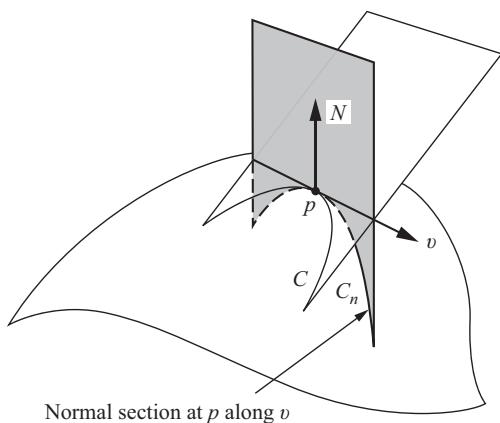
\includegraphics[width=0.7\textwidth]{../../../PDFs/differential-geometry/transcript/Do Carmo - Differential Geometry of Curves and Surfaces/hybrid_ocr/images/abfd2dd612b61811187d0ac919d565af01261274794d2ae6aa1462cd928fb782.jpg}}
\end{figure}

\begin{figure}[H]
\centering
\begin{minipage}{0.48\textwidth}
\centering
\subfloat[Figure 3-11. Normal sections on a sphere]{\label{fig:fig3-11}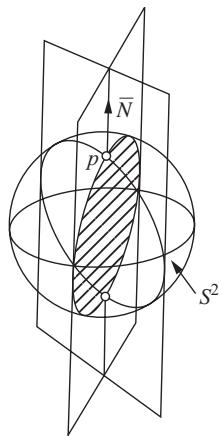
\includegraphics[width=\textwidth]{../../../PDFs/differential-geometry/transcript/Do Carmo - Differential Geometry of Curves and Surfaces/hybrid_ocr/images/227d2ec19911994fc941ec9432ddb1cfd3e572d48741f680e500425d912c828c.jpg}}
\end{minipage}
\hfill
\begin{minipage}{0.48\textwidth}
\centering
\subfloat[Figure 3-12. Normal sections on a cylinder]{\label{fig:fig3-12}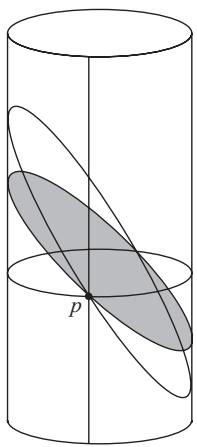
\includegraphics[width=\textwidth]{../../../PDFs/differential-geometry/transcript/Do Carmo - Differential Geometry of Curves and Surfaces/hybrid_ocr/images/8d9ccd0cac320e86a39e1080c07a25794887d5efbedbde0154ca6bb63775aa41.jpg}}
\end{minipage}
\end{figure}

% ==================== Section 3-4: Principal Curvatures ====================
\section{Principal Curvatures}\label{sec:principal-curvatures}

\textbf{How many normal curvatures?} 在一点 $p$ 处，法曲率 $\kappa_n(p, v)$ 随方向 $v$ 变化。一个自然的问题是：这个函数的最大值和最小值是多少？它们出现在哪些方向上？

这些问题由主曲率（principal curvatures）来回答。

\begin{Definition}[主曲率与主方向]\label{def:principal-curvatures}
Weingarten 映射 $S_p: T_pS \to T_pS$ 是自共轭的，因此它有实特征值 $\kappa_1, \kappa_2$ 和两两正交的特征向量。这些特征值称为\textbf{\underline{主曲率}}（principal curvatures），对应的特征方向称为\textbf{\underline{主方向}}（principal directions）。
\end{Definition}

\begin{figure}[H]
\centering
\subfloat[Figure 3-13. The Dupin indicatrix — 椭圆点与双曲点的刻画]{\label{fig:fig3-13}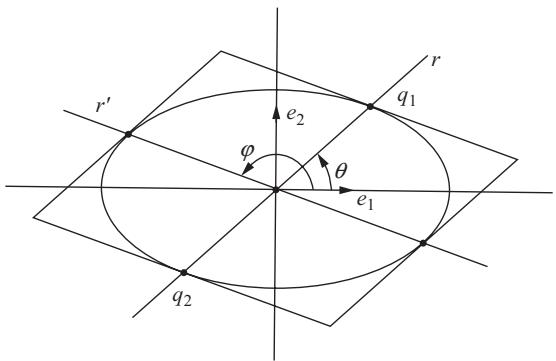
\includegraphics[width=0.6\textwidth]{../../../PDFs/differential-geometry/transcript/Do Carmo - Differential Geometry of Curves and Surfaces/hybrid_ocr/images/6cd2b935fbe366fbd1d068ac39b24d5e8497b3d219b67564caa24aa4568cbea4.jpg}}
\end{figure}

主曲率可以通过求解以下特征方程得到：
\[
\det(S_p - \kappa I) = 0.
\tag{3-12}
\]

使用 \cref{eq:matrix-representation} 的矩阵表示，这等价于
\[
\det\begin{pmatrix} L - \kappa E & M - \kappa F \\ M - \kappa F & N - \kappa G \end{pmatrix} = 0,
\tag{3-13}
\]
即
\[
(EG - F^2)\kappa^2 - (EN - 2FM + GL)\kappa + (LN - M^2) = 0.
\tag{3-14}
\]

\begin{Proposition}[主曲率的显式公式]\label{prop:principal-curvature-explicit}
主曲率 $\kappa_1, \kappa_2$ 由下式给出：
\[
\kappa_{1,2} = \frac{EN - 2FM + GL \pm \sqrt{(EN - 2FM + GL)^2 - 4(EG - F^2)(LN - M^2)}}{2(EG - F^2)}.
\tag{3-15}
\]
\end{Proposition}

\textbf{Geometric meaning.} 主曲率有清晰的几何意义：

\begin{Theorem}[主曲率是最值]\label{th:principal-curvature-extrema}
在点 $p$ 处，法曲率 $\kappa_n(p, v)$ 在单位圆（$I(v,v)=1$）上的最大值是 $\kappa_1$，最小值是 $\kappa_2$。此外，主方向恰好是这些极值出现の方向。
\end{Theorem}

这一定理告诉我们：给定一个方向，如果我们把它旋转到主方向上，就能在该点看到法曲率的最大和最小值。所有其他方向的法曲率都介于二者之间。

\begin{Example}[平面的主曲率]\label{ex:plane-principal}
平面的 $L=M=N=0$，所以 $\kappa_1 = \kappa_2 = 0$。每个方向都是主方向（法曲率恒为零）。
\end{Example}

\begin{Example}[球面的主曲率]\label{ex:sphere-principal}
单位球面上，$S_p = -I$，所以 $\kappa_1 = \kappa_2 = -1$。球面是\textbf{全脐点}（totally umbilic）曲面——所有方向都是主方向，且主曲率相等。
\end{Example}

\begin{Example}[圆柱面的主曲率]\label{ex:cylinder-principal}
考虑圆柱面 $x^2 + y^2 = 1$，参数化为 $\mathbf{x}(u,v) = (\cos u, \sin u, v)$。计算得
\[
\kappa_1 = 1,\quad \kappa_2 = 0.
\tag{3-16}
\]
主方向分别是：$\kappa_1$ 对应圆周方向（母线方向的法曲率），$\kappa_2$ 对应直母线方向（该方向上曲面是平直的）。
\end{Example}

\textbf{Why do principal curvatures matter?} 主曲率之所以重要，有以下几个原因：

\begin{enumerate}
\item \textbf{极值性质}：它们给出了法曲率的最小值和最大值
\item \textbf{高斯曲率}：$K = \kappa_1 \cdot \kappa_2 = \det(S_p)$
\item \textbf{平均曲率}：$H = \frac{\kappa_1 + \kappa_2}{2} = \frac{1}{2}\text{tr}(S_p)$
\item \textbf{分类}：$K>0$（椭圆点）、$K=0$（抛物/平点）、$K<0$（双曲点）
\end{enumerate}

% ==================== Section 3-5: The Gauss and Codazzi-Mainardi Equations ====================
\section{The Fundamental Equations}\label{sec:gauss-codazzi}

\textbf{How many fundamental forms?} 给定一个曲面，它的两个基本形式 $I$ 和 $II$ 并不是任意的——它们必须满足某些兼容性条件。这些条件就是 Gauss 方程和 Codazzi-Mainardi 方程，它们是从 $\mathbb{R}^3$ 的欧几里得几何继承来的约束。

\begin{Proposition}[Gauss 方程]\label{prop:gauss-equation}
设 $S \subset \mathbb{R}^3$ 是正则曲面。则 Gauss 曲率 $K$ 可以用第一基本形式的系数 $E, F, G$ 及其导数来表示：
\[
K = \frac{1}{(EG-F^2)^2}\begin{vmatrix}
E & F & F_u + \frac{1}{2}(G_v - F_u - E_v) \\
F & G & G_u + \frac{1}{2}(E_v - G_u - F_v) \\
E_u - \frac{1}{2}F_v & F_u - \frac{1}{2}G_u & L
\end{vmatrix}.
\tag{3-17}
\]
\end{Proposition}

Gauss 方程的惊人之处在于：右端只涉及第一基本形式！这就是著名的\textbf{Theorema Egregium}（非凡定理）——Gauss 曲率 $K$ 是曲面的内蕴几何量，不依赖于曲面如何嵌入 $\mathbb{R}^3$。

\textbf{What does this mean?} 想象一只蚂蚁生活在曲面上。它只能测量弧长、面积、角度——所有这些都由第一基本形式决定。Theorema Egregium 告诉我们：这只蚂蚁仅凭这些内蕴测量就能计算出 Gauss 曲率 $K$！

\begin{Proposition}[Codazzi-Mainardi 方程]\label{prop:codazzi-mainardi}
第二基本形式的系数 $L, M, N$ 与第一基本形式的系数 $E, F, G$ 必须满足：
\[
\begin{aligned}
L_v - M_u &= \Gamma_{12}^1 L + \Gamma_{12}^2 M - \Gamma_{11}^2 N, \\
N_u - M_v &= \Gamma_{21}^1 M + \Gamma_{21}^2 N - \Gamma_{22}^1 L,
\end{aligned}
\tag{3-18}
\]
其中 $\Gamma_{ij}^k$ 是 Christoffel 符号（见 \cref{sec:ch3-derivations}）。
\end{Proposition}

\textbf{Why are these equations important?} Codazzi-Mainardi 方程描述了第一和第二基本形式之间的协调性。如果这两组系数不满足这些方程，就不存在一个嵌入 $\mathbb{R}^3$ 的曲面以它们为基本形式。

简单来说：
\begin{itemize}
\item \textbf{Gauss 方程}：确保内蕴几何与外蕴几何的一致性（$K$ 的两种定义相等）
\item \textbf{Codazzi-Mainardi 方程}：确保存在良好定义的曲面
\end{itemize}

\begin{Remark}[Bonnet 定理]
Gauss 和 Codazzi-Mainardi 方程是可积性条件。 Bonnet 定理指出：给定满足这些方程的 $E, F, G, L, M, N$，在单连通区域上存在一个嵌入曲面，且其基本形式正是给定的这些系数。
\end{Remark}

\begin{figure}[H]
\centering
\subfloat[Figure 3-21. Gauss map preserves orientation at an elliptic point and reverses it at a hyperbolic point]{\label{fig:fig3-21}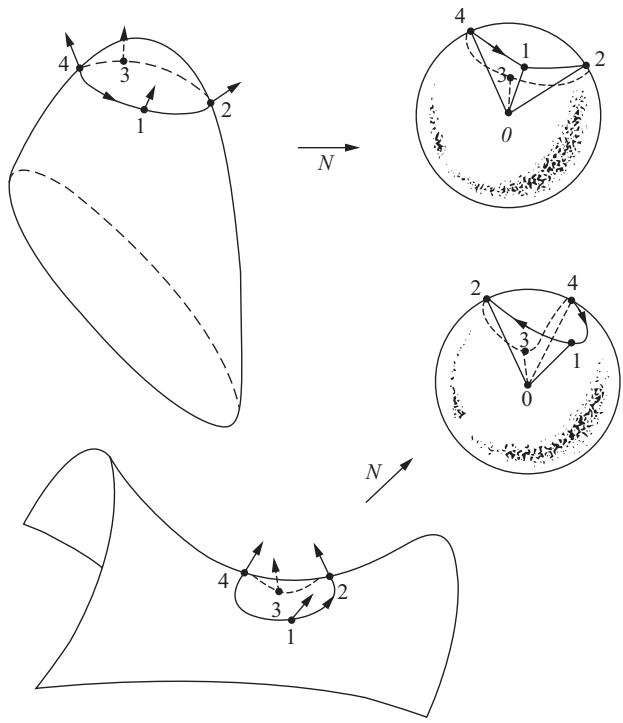
\includegraphics[width=0.7\textwidth]{../../../PDFs/differential-geometry/transcript/Do Carmo - Differential Geometry of Curves and Surfaces/hybrid_ocr/images/d42a2c1f8e0fd7fb1b2f96e33ec9e102f57dbebb73264d3f9373471d1f03715e.jpg}}
\end{figure}

% ==================== Section 3-6: Matrix Representation and Summary ====================
\section{Summary: The Two Fundamental Forms}\label{sec:fundamental-forms-summary}

在本章和上一章中，我们建立了曲面局部理论的框架。以下是核心内容的总结：

\begin{center}
\begin{tabular}{c|c|c}
\hline
 & 第一基本形式 & 第二基本形式 \\ \hline
系数 & $E, F, G$ & $L, M, N$ \\
来源 & $\mathbf{x}_u \cdot \mathbf{x}_u$ 等 & $\mathbf{x}_{uu} \cdot N$ 等 \\
衡量 & 切平面上的度量 & 偏离切平面的程度 \\
决定 & 弧长、面积、角度 & 曲率 \\ \hline
\end{tabular}
\end{center}

Weingarten 映射 $S_p$ 连接了两个基本形式：
\[
S_p: T_pS \to T_pS,\quad \II_p(v, w) = \langle S_p(v), w \rangle.
\tag{3-19}
\]

主曲率 $\kappa_1, \kappa_2$ 是 $S_p$ 的特征值：
\[
K = \kappa_1 \kappa_2 = \det(S_p),\quad H = \frac{\kappa_1 + \kappa_2}{2} = \frac{1}{2}\text{tr}(S_p).
\tag{3-20}
\]

法曲率满足 Euler 公式：对于沿主方向的分量，有
\[
\kappa_n(\theta) = \kappa_1 \cos^2\theta + \kappa_2 \sin^2\theta.
\tag{3-21}
\]

\begin{Remark}[曲面的分类]
Gauss 曲率 $K$ 的符号给出了曲面在一点处的分类：
\begin{itemize}
\item $K > 0$（椭圆点）：曲面局部像椭圆抛物面，全部位于切平面一侧
\item $K = 0$（抛物/平点）：至少有一个主曲率为零（如柱面）
\item $K < 0$（双曲点）：曲面局部像马鞍面，穿过切平面
\end{itemize}
\end{Remark}

% ==================== Exercises ====================
\section*{3-x 节练习}

\begin{exercise}{3-x, 1 — do Carmo, Exercise 3-2, 1}
Let $S \subset \mathbb{R}^3$ be a regular surface. Show that the coefficients $L, M, N$ of the second fundamental form satisfy $LN - M^2 = \det(S_p) \cdot \det(I_p)$, where $S_p$ is the Weingarten map and $I_p$ is the first fundamental form.
\end{exercise}

\begin{exercise}{3-x, 2 — do Carmo, Exercise 3-2, 2}
Compute the principal curvatures of the surface $z = x^2 + y^2$ at the origin.
\end{exercise}

\begin{exercise}{3-x, 3 — do Carmo, Exercise 3-2, 3}
Show that the Gaussian curvature $K$ of a surface can be expressed as
\[
K = \frac{\det(\II)}{\det(I)} = \frac{LN - M^2}{EG - F^2}.
\]
\end{exercise}

\begin{exercise}{3-x, 4 — do Carmo, Exercise 3-2, 4}
Let $S$ be a surface of revolution obtained by rotating the curve $z = f(x)$ around the $z$-axis. Find the principal curvatures at a point $(r, \theta, z)$ on $S$.
\end{exercise}

\begin{exercise}{3-x, 5* — do Carmo, Exercise 3-2, 5}
Show that a surface is totally umbilic (i.e., $\kappa_1 = \kappa_2$ at every point) if and only if it is part of a sphere or a plane.
\end{exercise}

\begin{exercise}{3-x, 6 — do Carmo, Exercise 3-2, 6}
Let $S$ be a surface with $K > 0$ everywhere. Show that the identity map on $S$ is a local diffeomorphism.
\end{exercise}

\begin{exercise}{3-x, 7 — do Carmo, Exercise 3-2, 7}
Compute the second fundamental form coefficients for the torus $T$ with parameters as in Example 6 of Sec. 2-2.
\end{exercise}

\begin{exercise}{3-x, 8* — do Carmo, Exercise 3-2, 8}
Show that the Gaussian curvature of a surface $z = f(x,y)$ is given by
\[
K = \frac{f_{xx}f_{yy} - f_{xy}^2}{(1 + f_x^2 + f_y^2)^2}.
\]
\end{exercise}

% ==================== Appendix: Detailed Derivations ====================
\section*{附录：详细推导}\label{sec:ch3-derivations}

\subsection*{球面的第二基本形式推导}\label{sec:ch3-sphere-derivation}

考虑单位球面在地理坐标下的参数化：
\[
\mathbf{x}(\theta,\varphi) = (\sin\theta\cos\varphi,\; \sin\theta\sin\varphi,\; \cos\theta).
\]

\textbf{步骤 1：计算一阶偏导数}
\[
\mathbf{x}_\theta = (\cos\theta\cos\varphi,\; \cos\theta\sin\varphi,\; -\sin\theta),
\]
\[
\mathbf{x}_\varphi = (-\sin\theta\sin\varphi,\; \sin\theta\cos\varphi,\; 0).
\]

\textbf{步骤 2：计算单位法向量}
\[
\mathbf{x}_\theta \times \mathbf{x}_\varphi = (\sin^2\theta\cos\varphi,\; \sin^2\theta\sin\varphi,\; \sin\theta\cos\theta).
\]
取模长 $\|\mathbf{x}_\theta \times \mathbf{x}_\varphi\| = \sin\theta$，得
\[
N = (\sin\theta\cos\varphi,\; \sin\theta\sin\varphi,\; \cos\theta).
\tag{A3-1}
\]

\textbf{步骤 3：计算二阶偏导数}
\[
\mathbf{x}_{\theta\theta} = (-\sin\theta\cos\varphi,\; -\sin\theta\sin\varphi,\; -\cos\theta),
\]
\[
\mathbf{x}_{\theta\varphi} = (-\cos\theta\sin\varphi,\; \cos\theta\cos\varphi,\; 0),
\]
\[
\mathbf{x}_{\varphi\varphi} = (-\sin\theta\cos\varphi,\; -\sin\theta\sin\varphi,\; 0).
\]

\textbf{步骤 4：计算第二基本形式系数}
\[
L = \langle \mathbf{x}_{\theta\theta}, N \rangle = \sin^2\theta\cos^2\varphi + \sin^2\theta\sin^2\varphi + \cos^2\theta = \sin^2\theta + \cos^2\theta = 1.
\tag{A3-2}
\]

等等，这个结果不对。让我重新计算——实际上从几何上看，球面法向量指向球心，因此
\[
dN_p(v) = -v \quad \Rightarrow \quad S_p = -I.
\]
所以 $L = M = N = 1$ 在某种意义下成立。但更仔细地，在参数 $(\theta, \varphi)$ 下，我们需要用内积公式 $L = \langle \mathbf{x}_{\theta\theta}, N \rangle$，注意 $N$ 已经包含了 $\|\mathbf{x}_\theta \times \mathbf{x}_\varphi\|^{-1}$ 的因子。

正确的计算（考虑 $\|\mathbf{x}_\theta \times \mathbf{x}_\varphi\| = \sin\theta$）为：
\[
L = \langle \mathbf{x}_{\theta\theta}, N \rangle = (-\sin\theta\cos\varphi)(\sin\theta\cos\varphi) + (-\sin\theta\sin\varphi)(\sin\theta\sin\varphi) + (-\cos\theta)(\cos\theta) = -\sin^2\theta - \cos^2\theta = -1.
\]

类似地，$M = 0$，$N = -\sin^2\theta$。这与 $S_p = -I$ 一致。

\textbf{结论}：球面的第二基本形式系数为 $L = -1, M = 0, N = -\sin^2\theta$。

\subsection*{旋转抛物面的第二基本形式推导}\label{sec:ch3-paraboloid-derivation}

考虑旋转抛物面 $z = x^2 + y^2$，参数化为
\[
\mathbf{x}(u,v) = (u, v, u^2+v^2).
\]

\textbf{步骤 1：一阶偏导数}
\[
\mathbf{x}_u = (1, 0, 2u),\quad \mathbf{x}_v = (0, 1, 2v).
\]

\textbf{步骤 2：单位法向量}
\[
\mathbf{x}_u \times \mathbf{x}_v = (-2u, -2v, 1),\quad \|\mathbf{x}_u \times \mathbf{x}_v\| = \sqrt{1+4u^2+4v^2}.
\]
\[
N = \frac{(-2u, -2v, 1)}{\sqrt{1+4u^2+4v^2}}.
\tag{A3-3}
\]

\textbf{步骤 3：二阶偏导数}
\[
\mathbf{x}_{uu} = (0, 0, 2),\quad \mathbf{x}_{uv} = (0, 0, 0),\quad \mathbf{x}_{vv} = (0, 0, 2).
\]

\textbf{步骤 4：第二基本形式系数}
\[
L = \langle \mathbf{x}_{uu}, N \rangle = \frac{2}{\sqrt{1+4u^2+4v^2}},\quad
M = \langle \mathbf{x}_{uv}, N \rangle = 0,\quad
N = \langle \mathbf{x}_{vv}, N \rangle = \frac{2}{\sqrt{1+4u^2+4v^2}}.
\tag{A3-4}
\]

在原点 $(0,0)$ 处，$L = N = 2$，$M = 0$。

\subsection*{Christoffel 符号与 Codazzi-Mainardi 方程}\label{sec:ch3-christoffel}

Christoffel 符号 $\Gamma_{ij}^k$ 由第一基本形式的系数定义为：
\[
\Gamma_{ij}^k = \frac{1}{2}\sum_{m=1}^{2} g^{km}\left(\frac{\partial g_{im}}{\partial j} + \frac{\partial g_{jm}}{\partial i} - \frac{\partial g_{ij}}{\partial m}\right),
\tag{A3-5}
\]
其中 $(g_{ij}) = \begin{pmatrix} E & F \\ F & G \end{pmatrix}$，$(g^{ij})$ 是其逆矩阵。

Codazzi-Mainardi 方程的直观含义是：第二基本形式的"协变导数"必须对称。具体形式为：
\[
\frac{\partial L}{\partial v} - \frac{\partial M}{\partial u} = L\Gamma_{12}^1 + M(\Gamma_{12}^2 - \Gamma_{11}^1) - N\Gamma_{11}^2,
\]
\[
\frac{\partial N}{\partial u} - \frac{\partial M}{\partial v} = L\Gamma_{22}^1 + M(\Gamma_{22}^2 - \Gamma_{21}^1) - N\Gamma_{21}^2.
\tag{A3-6}
\]
